% ============================================================
%  RELATÓRIO — ARQUITETURAS DE ALTO DESEMPENHO
%  Prática 6: Jogo da Vida de Conway em FPGA com Saída VGA
%  Normas para Elaboração de Relatórios ver 4 (2026)
%  Universidade Federal de São Carlos (UFSCar)
% ============================================================
\documentclass[12pt, a4paper]{article}

% --- Codificação e idioma ---
\usepackage[utf8]{inputenc}
\usepackage[T1]{fontenc}
\usepackage[brazil]{babel}
\usepackage{amsmath}
\usepackage{amssymb}
\usepackage{multirow}

% --- Fonte Times New Roman ---
\usepackage{mathptmx}

% --- Geometria da página ---
\usepackage[
top=2.5cm,
bottom=2.5cm,
left=3.0cm,
right=3.0cm
]{geometry}

% --- Espaçamento entre linhas ---
\usepackage{setspace}
\onehalfspacing

% --- Indentação do parágrafo ---
\usepackage{indentfirst}
\setlength{\parindent}{1.25cm}

% --- Pacotes gráficos e de figuras ---
\usepackage{graphicx}
\usepackage{float}

% --- Tabelas ---
\usepackage{booktabs}
\usepackage{array}
\usepackage{longtable}

% --- Listagens de código ---
\usepackage{listings}
\usepackage{xcolor}

\lstdefinestyle{verilog}{
	language=Verilog,
	basicstyle=\ttfamily\small,
	keywordstyle=\color{blue}\bfseries,
	commentstyle=\color{gray}\itshape,
	stringstyle=\color{teal},
	numbers=left,
	numberstyle=\tiny\color{gray},
	stepnumber=1,
	numbersep=8pt,
	frame=single,
	breaklines=true,
	breakatwhitespace=true,
	columns=flexible,
	keepspaces=true,
	captionpos=b,
	morekeywords={module,endmodule,input,output,reg,wire,always,begin,end,
		posedge,negedge,if,else,case,endcase,assign,parameter,
		localparam,integer,initial,for,while,task,endtask,defparam}
}

% --- Numeração de seções ---
\setcounter{secnumdepth}{3}

% --- Cabeçalho e rodapé ---
\usepackage{fancyhdr}
\setlength{\headheight}{14pt}
\pagestyle{fancy}
\fancyhf{}
\fancyhead[R]{\small Arquiteturas de Alto Desempenho --- Relatório}
\fancyfoot[C]{\thepage}
\renewcommand{\headrulewidth}{0.4pt}

% --- Hiperlinks (DEVE ser o último pacote) ---
\usepackage[hidelinks]{hyperref}

% ============================================================
%  INÍCIO DO DOCUMENTO
% ============================================================
\begin{document}
	
	\thispagestyle{empty}
	
	% ============================================================
	%  CAPA
	% ============================================================
	\begin{titlepage}
		\centering
		
		\noindent\rule{\textwidth}{0.8pt}\\[0.2cm]
		{\large \textbf{UNIVERSIDADE FEDERAL DE SÃO CARLOS}}\\[0.15cm]
		{\normalsize Centro de Ciências Exatas e Tecnologia}\\[0.15cm]
		{\normalsize Departamento de Computação}\\[0.15cm]
		
		\vspace{0pt plus 0.35fill}
		
		{\large \textbf{Laboratório de Arquiteturas de Alto Desempenho}}\\[0.4cm]
		{\large Prática 6 --- Jogo da Vida de Conway em FPGA\\[0.2cm]
			com Arquitetura Pipeline e Saída VGA}\\[1.0cm]
		{\normalsize Professor: \textit{Dr. Emerson Carlos Pedrino}}\\
		
		\vspace{0pt plus 0.65fill}
		
		\begin{center}
			{\normalsize \textit{Pedro Augusto Faria} \ (RA: \textit{821124})}\\[0.15cm]
			{\normalsize Curso: \textit{Engenharia da Computação}}\\[0.15cm]
		\end{center}
		
	\end{titlepage}
	
	\setcounter{page}{1}
	
	% ============================================================
	%  SEÇÃO 1 — INTRODUÇÃO
	% ============================================================
	\section{Introdução}
	
	O Jogo da Vida (\textit{Game of Life}), criado pelo matemático britânico John
	Horton Conway em 1970, é um autômato celular bidimensional que simula a evolução
	de uma população de células dispostas em uma grade regular. Apesar de sua
	formulação extremamente simples --- quatro regras de transição aplicadas a uma
	vizinhança de 8 células --- o sistema exibe comportamento emergente de notável
	complexidade, incluindo estruturas estáveis, osciladores, planadores
	(\textit{gliders}) e até mesmo estruturas computacionalmente universais (capazes
	de simular uma máquina de Turing).
	
	Do ponto de vista das arquiteturas de alto desempenho, o Jogo da Vida é um
	problema paradigmático para o estudo de paralelismo espacial e temporal. A
	atualização de cada célula depende exclusivamente dos valores de seus 8 vizinhos
	no ciclo anterior, sem qualquer dependência de dados entre células distintas na
	mesma geração. Esta independência torna o problema \textit{embaraçosamente
		paralelo} e ideal para implementação em hardware reconfigurável (FPGA), onde
	todas as células podem ser avaliadas simultaneamente em um único ciclo de clock,
	em contraste com uma implementação sequencial em software que percorreria as
	$64 \times 64 = 4096$ células uma a uma.
	
	Esta prática implementa o Jogo da Vida em uma grade de 64$\times$64 células
	na FPGA Altera DE1 (Cyclone II), utilizando o ambiente Quartus Prime. O sistema
	exibe a evolução do autômato em tempo real em um monitor VGA de resolução
	640$\times$480 pixels. O usuário pode controlar a velocidade de evolução
	(automática ou manual por botão), selecionar o padrão inicial (padrão
	\textit{hardcoded} ou carregado de ROM) e avançar geração a geração
	interativamente.
	
	\subsection{Fundamentação Teórica}
	
	\subsubsection{Autômatos Celulares e o Jogo da Vida}
	
	Um autômato celular é um modelo computacional discreto no espaço, no tempo e
	nos estados. O Jogo da Vida de Conway opera sobre uma grade bidimensional de
	células, cada uma podendo estar \textit{viva} (1) ou \textit{morta} (0). A cada
	geração (passo de tempo), todas as células são atualizadas simultaneamente de
	acordo com as seguintes regras, baseadas no número $n$ de vizinhos vivos na
	vizinhança de Moore (os 8 pixels adjacentes):
	
	\begin{enumerate}
		\item Uma célula \textbf{viva} com $n < 2$ vizinhos vivos \textbf{morre}
		(subpopulação);
		\item Uma célula \textbf{viva} com $n \in \{2, 3\}$ vizinhos vivos
		\textbf{sobrevive} para a próxima geração;
		\item Uma célula \textbf{viva} com $n > 3$ vizinhos vivos \textbf{morre}
		(superpopulação);
		\item Uma célula \textbf{morta} com $n = 3$ vizinhos vivos \textbf{nasce}
		(reprodução).
	\end{enumerate}
	
	Estas quatro regras podem ser expressas compactamente como:
	
	\begin{equation}
		c'(i,j) =
		\begin{cases}
			1 & \text{se } c(i,j) = 1 \text{ e } n(i,j) \in \{2, 3\} \\
			1 & \text{se } c(i,j) = 0 \text{ e } n(i,j) = 3 \\
			0 & \text{caso contrário}
		\end{cases}
		\label{eq:regras}
	\end{equation}
	
	\noindent onde $c(i,j)$ é o estado da célula na linha $i$, coluna $j$ na
	geração atual, $c'(i,j)$ é seu estado na próxima geração, e $n(i,j)$ é o
	número de vizinhos vivos:
	
	\begin{equation}
		n(i,j) = \sum_{\substack{l \in \{-1,0,1\} \\ k \in \{-1,0,1\} \\ (l,k) \neq (0,0)}} c(i+l,\; j+k)
		\label{eq:vizinhos}
	\end{equation}
	
	\subsubsection{Padrão Inicial: Canhão de Planadores de Gosper}
	
	O padrão \textit{hardcoded} implementado no sistema é o \textbf{Canhão de
		Planadores de Gosper} (\textit{Gosper Glider Gun}), descoberto por Bill Gosper
	em 1970 em resposta a um desafio proposto pelo próprio Conway. É o primeiro
	padrão descoberto com crescimento ilimitado de população: a estrutura oscila
	periodicamente com período 30 e emite um novo planador (\textit{glider}) a cada
	30 gerações, resultando em crescimento linear da população ao longo do tempo.
	
	O planador (\textit{glider}) é a menor estrutura periódica que se translada
	pelo espaço: completa um ciclo em 4 gerações e desloca-se 1 célula na diagonal
	a cada ciclo, com velocidade de $c/4$ (um quarto da velocidade máxima de
	propagação de informação na grade). O canhão de Gosper ocupa uma região de
	aproximadamente $36 \times 9$ células e é composto por duas estruturas oscilantes
	(\textit{pentadecathlons} modificados) e dois blocos estáticos que refletem os
	planadores gerados.
	
	\subsubsection{Representação da Grade em Hardware}
	
	A grade 64$\times$64 é armazenada como um vetor de 4096 bits:
	\texttt{current\_grid[4095:0]}, onde a célula na linha $i$ (0-indexada) e coluna
	$j$ está no bit de índice $i \times 64 + j$. Esta representação planificada
	(\textit{row-major}) é natural para registradores em FPGA e permite que o acesso
	a qualquer célula seja realizado por aritmética de índice simples, sintetizável
	em lógica combinacional.
	
	\subsubsection{Divisão de Clock e Controle de Velocidade}
	
	O clock principal da placa DE1 é de 50~MHz, correspondendo a um período de
	20~ns. Para que o Jogo da Vida evolua em velocidade visível ao olho humano
	(da ordem de $0{,}1$ a $10$ gerações por segundo), é necessário dividir este
	clock por um fator elevado. O módulo \texttt{clock\_divider} conta 5.000.000
	ciclos de clock (0,1 segundo) antes de emitir um pulso de atualização
	(\texttt{update\_pulse}) de 1 ciclo de duração. Isso resulta em uma taxa de
	atualização de 10 gerações por segundo no modo automático.
	
	No modo manual, o botão \texttt{KEY[1]} gera um pulso a cada acionamento por
	meio do módulo \texttt{button\_pulse}, que detecta a transição de descida
	(\textit{falling edge}) do botão. O módulo \texttt{pulse\_mux} seleciona entre
	os dois modos de operação por meio do \textit{switch} \texttt{SW[1]}.
	
	\subsubsection{Mapeamento da Grade para o Monitor VGA}
	
	A grade 64$\times$64 é exibida no monitor VGA 640$\times$480 com cada célula
	ocupando uma região retangular de $10 \times 7$ pixels (largura $\times$ altura).
	Isso resulta em uma área de exibição de $640 \times 448$ pixels, que cabe dentro
	do quadro VGA ativo. O módulo \texttt{LifeToVGAMono2} mapeia as coordenadas de
	pixel do controlador VGA para o índice de célula correspondente na grade:
	
	\begin{equation}
		\text{col\_index} = \left\lfloor \frac{\texttt{pixel\_column}}{10} \right\rfloor, \qquad
		\text{row\_index} = \left\lfloor \frac{\texttt{pixel\_row}}{7} \right\rfloor
		\label{eq:mapeamento}
	\end{equation}
	
	O pixel de saída recebe o valor da célula $\texttt{grid}[\text{row\_index}
	\times 64 + \text{col\_index}]$. Fora da região de interesse
	($\texttt{pixel\_column} \geq 640$ ou $\texttt{pixel\_row} \geq 448$), o pixel
	de habilitação (\texttt{pixel\_enable}) é desativado e a saída é forçada a $0$.
	
	\subsubsection{Carregamento de Padrão por ROM}
	
	Quando \texttt{SW[0] = 0} (modo ROM), o sistema carrega o padrão inicial da
	memória ROM (\texttt{rom}) após o reset. O módulo \texttt{GameOfLife2} entra no
	estado de carregamento (\texttt{loading = 1}) e percorre sequencialmente os
	4096 endereços da ROM, copiando cada bit para a posição correspondente em
	\texttt{current\_grid}. O processo leva 4096 ciclos de clock ($\approx 82\,\mu$s
	a 50~MHz) e é completamente transparente ao usuário.
	
	\subsection{Objetivos}
	
	\begin{itemize}
		\item Implementar o Jogo da Vida de Conway em uma grade 64$\times$64 em
		hardware Verilog, executando na FPGA Altera DE1;
		\item Aplicar a arquitetura pipeline para atualização do estado da grade
		a cada geração, com sincronismo controlado por divisor de clock;
		\item Exibir a evolução do autômato em tempo real em monitor VGA
		640$\times$480, com mapeamento correto de células para pixels;
		\item Implementar controle interativo: modo automático (10 gen/s) e manual
		(avanço por botão), seleção de padrão inicial (ROM ou \textit{hardcoded}),
		e reset por botão;
		\item Demonstrar o comportamento do Canhão de Planadores de Gosper como
		padrão \textit{hardcoded} e de padrões arbitrários carregados de ROM.
	\end{itemize}
	
	\subsection{Metodologia}
	
	O projeto foi desenvolvido no ambiente Quartus Prime (Versão 24.1std.0 Build 1077,
	Lite Edition), com módulos descritos em Verilog e integrados por diagrama
	esquemático BDF. O módulo \texttt{VGA\_SYNC} foi fornecido pelo professor. Os
	módulos desenvolvidos foram sintetizados para a FPGA Cyclone II EP2C20F484C7
	da placa Altera DE1, com pinagem definida pelo arquivo de pinos oficial.
	
	% ============================================================
	%  SEÇÃO 2 — DESENVOLVIMENTO TEÓRICO
	% ============================================================
	\section{Desenvolvimento Teórico}
	
	\subsection{Análise das Regras do Jogo da Vida em Hardware}
	
	A implementação das regras do Jogo da Vida em hardware digital requer, para cada
	célula $(i,j)$, o cálculo da soma dos 8 vizinhos e a avaliação da função de
	transição. Para uma grade binária (células de 1 bit), a soma dos 8 vizinhos
	é um inteiro no intervalo $[0, 8]$, representável em 4 bits. A função de
	transição é então:
	
	\begin{equation}
		c'(i,j) = \bigl[c(i,j) \wedge (n=2 \vee n=3)\bigr]
		\vee \bigl[\neg c(i,j) \wedge (n=3)\bigr]
		\label{eq:hw_rule}
	\end{equation}
	
	\noindent que simplifica para:
	
	\begin{equation}
		c'(i,j) = (n = 3) \vee \bigl[c(i,j) \wedge (n = 2)\bigr]
		\label{eq:hw_rule_simplified}
	\end{equation}
	
	Esta expressão booleana é sintetizável diretamente em lógica combinacional:
	um somador de 8 bits de 1 bit cada, seguido de um comparador e duas portas
	lógicas. Em hardware paralelo, todas as 4096 células são avaliadas
	simultaneamente, completando uma geração em um único ciclo de clock (após a
	latência do combinacional).
	
	Na implementação em Verilog adotada, o laço \texttt{for} aninhado sobre todas
	as células é expandido pelo sintetizador em lógica paralela para a grade completa,
	confirmando o caráter massivamente paralelo da arquitetura.
	
	\subsection{Condições de Fronteira}
	
	A grade 64$\times$64 implementada utiliza \textbf{fronteiras fixas}: as células
	das bordas (linha 0, linha 63, coluna 0 e coluna 63) são mantidas no estado da
	geração anterior sem aplicar as regras de transição. Esta é uma simplificação
	de implementação que evita o tratamento de casos especiais de vizinhança nas
	bordas e a lógica de \textit{wrapping} toroidal. Para o Canhão de Gosper
	posicionado no interior da grade (linhas 10--20, colunas 0--35), a borda fixa
	não afeta o comportamento do padrão por muitas gerações, até que os planadores
	gerados atinjam a borda e sejam absorvidos.
	
	\subsection{Arquitetura de Atualização: Paralelismo Massivo vs. Pipeline}
	
	Existem dois paradigmas principais para implementar a atualização do Jogo da
	Vida em FPGA:
	
	\textbf{Paralelo puro:} todas as células são calculadas simultaneamente em
	lógica combinacional, e o resultado é registrado em um único flip-flop de
	habilitação (\texttt{update\_pulse}). Esta é a abordagem adotada neste projeto.
	O custo é elevado em termos de lógica combinacional (4096 somadores + 4096
	comparadores), mas o throughput é máximo: 1 geração por ciclo de clock habilitado.
	
	\textbf{Pipeline seriado:} as células são calculadas em sequência por um único
	núcleo de processamento com \textit{line buffers}, similar ao pipeline da Prática
	anterior. O custo de lógica é mínimo, mas o throughput é de 1 célula por ciclo,
	exigindo $4096$ ciclos por geração.
	
	O projeto utiliza a abordagem paralela pura, onde o vetor \texttt{next[4095:0]}
	é calculado inteiramente em lógica combinacional dentro do bloco \texttt{always}
	e registrado atomicamente no flanco de subida do clock quando \texttt{update\_pulse}
	é ativo. A taxa de atualização é controlada externamente pelo \texttt{clock\_divider},
	que determina a cadência das gerações.
	
	\subsection{Sincronismo entre Atualização da Grade e Varredura VGA}
	
	Um aspecto crítico do projeto é a coexistência de dois processos assíncronos:
	a atualização da grade (a 10~Hz ou sob controle manual) e a varredura VGA (a
	60~Hz, pixel clock $\approx 25$~MHz). Ambos leem \texttt{current\_grid}
	simultaneamente, mas apenas o módulo \texttt{GameOfLife2} escreve neste registro.
	
	A atualização ocorre em um único ciclo de clock (escrita síncrona no flanco de
	subida quando \texttt{update\_pulse = 1}), enquanto a leitura pelo módulo
	\texttt{LifeToVGAMono2} é combinacional (sem clock). Como a taxa de atualização
	(10~Hz) é vastamente inferior à taxa de quadros VGA (60~Hz), a probabilidade de
	uma atualização ocorrer durante a varredura de um quadro é de aproximadamente
	$1/(50\,\text{MHz} / 10\,\text{Hz}) \approx 2 \times 10^{-7}$ por ciclo, tornando
	artefatos visuais de \textit{tearing} praticamente imperceptíveis.
	
	\subsection{Mapeamento de Escala para VGA}
	
	O fator de escala inteiro (10 pixels por coluna, 7 pixels por linha) foi escolhido
	para maximizar o uso da tela VGA 640$\times$480:
	
	\begin{equation}
		64 \times 10 = 640 \text{ pixels de largura} \qquad \text{(uso total)}
		\label{eq:escala_h}
	\end{equation}
	
	\begin{equation}
		64 \times 7 = 448 \text{ pixels de altura} \qquad \text{(32 pixels não utilizados)}
		\label{eq:escala_v}
	\end{equation}
	
	A divisão inteira por potências de 2 não é aplicável diretamente (10 e 7 não
	são potências de 2), de forma que o Quartus Prime sintetiza divisores combinacionais
	para estas constantes. Como as entradas \texttt{pixel\_column} e \texttt{pixel\_row}
	são sinais de 10 bits com valores máximos de 639 e 479, os quocientes
	\texttt{col\_index} e \texttt{row\_index} têm no máximo 6 bits ($0$ a $63$),
	cobrindo exatamente o intervalo de índices da grade.
	
	% ============================================================
	%  SEÇÃO 3 — DESENVOLVIMENTO PRÁTICO
	% ============================================================
	\section{Desenvolvimento Prático}
	\label{sec:pratico}
	
	\subsection{Ambiente de Desenvolvimento}
	
	\begin{table}[H]
		\centering
		\caption{Especificações do ambiente de desenvolvimento.}
		\label{tab:ambiente}
		\begin{tabular}{ll}
			\toprule
			\textbf{Parâmetro}        & \textbf{Valor}                                     \\
			\midrule
			Placa FPGA                & Altera DE1 (Cyclone II EP2C20F484C7)               \\
			Ferramenta EDA            & Quartus Prime 24.1std.0 Build 1077 (Lite Edition)  \\
			Linguagem principal       & Verilog                                            \\
			Linguagem auxiliar        & VHDL (\texttt{VGA\_SYNC}, fornecido)               \\
			Clock da placa            & 50~MHz                                             \\
			Pixel clock VGA           & $\approx$25,175~MHz                                \\
			Resolução VGA             & 640$\times$480 @ 60~Hz                             \\
			Resolução da grade        & 64$\times$64 células, 1 bit/célula                 \\
			Tamanho da célula na tela & 10$\times$7 pixels (col $\times$ lin)              \\
			Taxa de atualização       & 10 gerações/s (automático) ou manual               \\
			Sistema Operacional       & Ubuntu 24.04.4 LTS (Kubuntu)                       \\
			\bottomrule
		\end{tabular}
	\end{table}
	
	\subsection{Estrutura Geral do Projeto e Diagrama de Blocos}
	
	O sistema é integrado pelo módulo \textit{top-level} \texttt{vga\_filtro} por
	meio do editor de esquemáticos BDF do Quartus Prime. A Figura~\ref{fig:top_bdf}
	apresenta o diagrama BDF representativo do sistema completo.
	
	\begin{figure}[H]
		\centering
		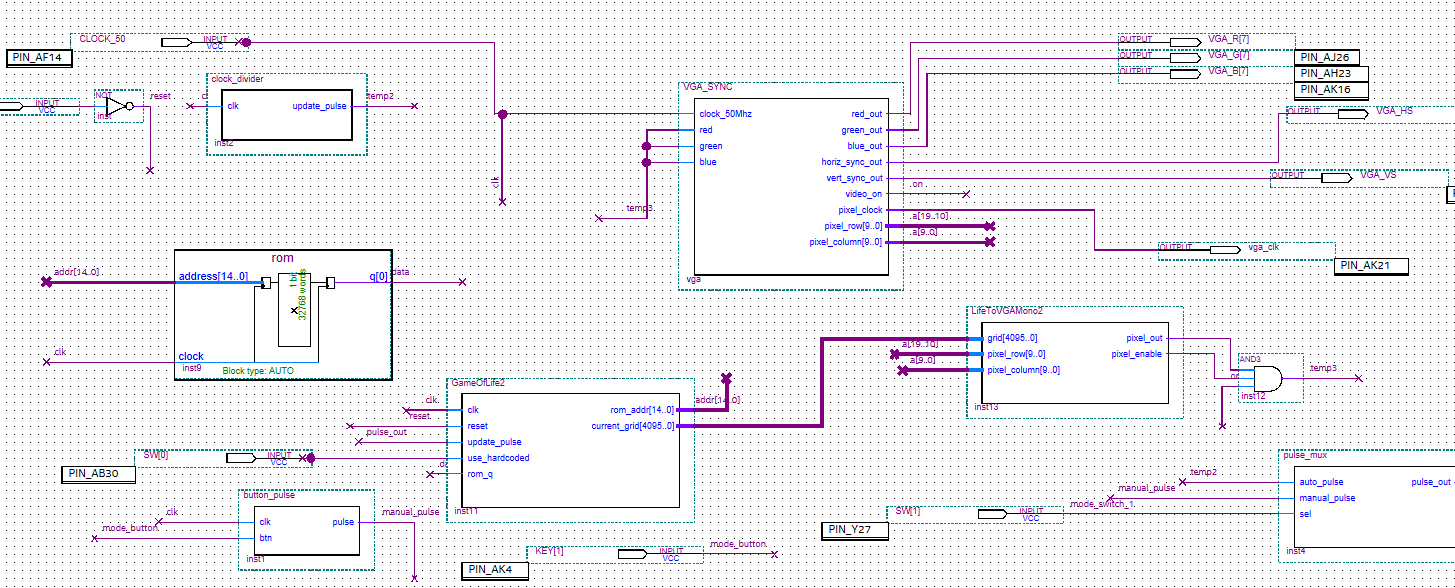
\includegraphics[width=1.0\textwidth]{top_bdf_representative_only_icons_too_small_to_see.png}
		\caption{Diagrama BDF do módulo \textit{top-level} \texttt{vga\_filtro} no
			Quartus Prime, evidenciando a interligação de todos os componentes
			do sistema do Jogo da Vida.}
		\label{fig:top_bdf}
	\end{figure}
	
	Os módulos que compõem o sistema são:
	
	\begin{itemize}
		\item \texttt{VGA\_SYNC} --- Controlador VGA (VHDL, fornecido); gera
		\texttt{HSync}, \texttt{VSync}, \texttt{video\_on}, \texttt{pixel\_clock}
		e os contadores de coordenadas \texttt{pixel\_column}/\texttt{pixel\_row};
		\item \texttt{GameOfLife2} --- Núcleo do autômato celular; armazena e atualiza
		a grade 64$\times$64, com suporte a reset, carregamento de ROM e
		padrão \textit{hardcoded};
		\item \texttt{LifeToVGAMono2} --- Conversor grade $\to$ VGA; mapeia as
		coordenadas de pixel para o índice de célula e habilita a saída;
		\item \texttt{clock\_divider} --- Divisor de clock; gera pulso de atualização
		a 10~Hz (a cada 5.000.000 ciclos de 50~MHz);
		\item \texttt{button\_pulse} --- Detector de borda de descida do botão;
		gera pulso de 1 ciclo por acionamento de \texttt{KEY[1]};
		\item \texttt{pulse\_mux} --- Multiplexador de pulso; seleciona entre
		atualização automática e manual por \texttt{SW[1]};
		\item \texttt{rom} --- Memória ROM com padrão inicial alternativo de
		4096 bits (1 bit por endereço).
	\end{itemize}
	
	\subsection{Módulo \texttt{GameOfLife2} --- Núcleo do Autômato Celular}
	
	O módulo \texttt{GameOfLife2} é o componente central do sistema. Ele armazena
	o estado completo da grade 64$\times$64 no registrador \texttt{current\_grid[4095:0]}
	e implementa três modos de operação: inicialização com padrão \textit{hardcoded}
	(Canhão de Gosper), carregamento da ROM e atualização pela regra do Jogo da Vida.
	
	\begin{lstlisting}[style=verilog, caption={\texttt{GameOfLife2.v} --- Núcleo do autômato celular com suporte a reset, carregamento de ROM e atualização paralela da grade 64$\times$64.}, label={lst:gameoflife}]
		module GameOfLife2 (
		input clk,
		input reset,
		input update_pulse,
		input use_hardcoded,
		input rom_q,
		output reg [14:0] rom_addr,
		output reg [4095:0] current_grid
		);
		integer i, j, l, c, count;
		reg [4095:0] next;
		reg [11:0] load_addr;
		reg loading;
		
		task set_hardcoded;
		begin
		current_grid = 0;
		// Canhao de Planadores de Gosper
		current_grid[10*64 + 24] = 1;
		current_grid[11*64 + 22] = 1; current_grid[11*64 + 24] = 1;
		current_grid[12*64 + 12] = 1; current_grid[12*64 + 13] = 1;
		current_grid[12*64 + 20] = 1; current_grid[12*64 + 21] = 1;
		current_grid[12*64 + 34] = 1; current_grid[12*64 + 35] = 1;
		current_grid[13*64 + 11] = 1; current_grid[13*64 + 15] = 1;
		current_grid[13*64 + 20] = 1; current_grid[13*64 + 21] = 1;
		current_grid[13*64 + 34] = 1; current_grid[13*64 + 35] = 1;
		current_grid[14*64 + 0]  = 1; current_grid[14*64 + 1]  = 1;
		current_grid[14*64 + 10] = 1; current_grid[14*64 + 16] = 1;
		current_grid[14*64 + 20] = 1; current_grid[14*64 + 21] = 1;
		current_grid[15*64 + 0]  = 1; current_grid[15*64 + 1]  = 1;
		current_grid[15*64 + 10] = 1; current_grid[15*64 + 14] = 1;
		current_grid[15*64 + 16] = 1; current_grid[15*64 + 17] = 1;
		current_grid[15*64 + 22] = 1; current_grid[15*64 + 24] = 1;
		current_grid[16*64 + 10] = 1; current_grid[16*64 + 16] = 1;
		current_grid[17*64 + 11] = 1; current_grid[17*64 + 15] = 1;
		current_grid[18*64 + 12] = 1; current_grid[18*64 + 13] = 1;
		current_grid[19*64 + 22] = 1; current_grid[19*64 + 24] = 1;
		current_grid[20*64 + 23] = 1;
		end
		endtask
		
		initial begin
		set_hardcoded;
		loading = 0;
		load_addr = 0;
		rom_addr = 0;
		end
		
		always @(posedge clk) begin
		if (reset) begin
		// Resetar para padrao hardcoded ou iniciar carga da ROM
		loading <= ~use_hardcoded;
		load_addr <= 0;
		rom_addr <= 0;
		if (use_hardcoded) begin
		// Inicializacao sequencial por atribuicoes nao-bloqueantes
		current_grid <= 0;
		current_grid[10*64 + 24] <= 1;
		// ... (demais celulas do Canhao de Gosper)
		current_grid[20*64 + 23] <= 1;
		end else
		current_grid <= 0;
		end else if (loading) begin
		// Carregamento serial da ROM: 1 bit por ciclo de clock
		if (load_addr > 0)
		current_grid[load_addr - 1] <= rom_q;
		rom_addr <= {3'b000, load_addr};
		if (load_addr == 12'd4095) begin
		current_grid[4094] <= rom_q;
		loading <= 0;
		end else
		load_addr <= load_addr + 1;
		end else if (update_pulse) begin
		// Atualizacao paralela: calcular proxima geracao
		next = 0;
		// Bordas fixas: copiar sem aplicar regras
		for (i = 0; i < 64; i = i + 1) begin
		next[i*64 + 0]  = current_grid[i*64 + 0];
		next[i*64 + 63] = current_grid[i*64 + 63];
		end
		for (j = 0; j < 64; j = j + 1) begin
		next[0*64 + j]  = current_grid[0*64 + j];
		next[63*64 + j] = current_grid[63*64 + j];
		end
		// Interior: aplicar regras do Jogo da Vida
		for (i = 1; i < 63; i = i + 1) begin
		for (j = 1; j < 63; j = j + 1) begin
		count = 0;
		for (l = 0; l < 3; l = l + 1)
		for (c = 0; c < 3; c = c + 1)
		if (!(l == 1 && c == 1))
		count = count +
		current_grid[(i+l-1)*64 + (j+c-1)];
		if (current_grid[i*64 + j])
		next[i*64+j] = (count==2||count==3) ? 1'b1 : 1'b0;
		else
		next[i*64+j] = (count==3) ? 1'b1 : 1'b0;
		end
		end
		current_grid <= next;
		end
		end
		endmodule
	\end{lstlisting}
	
	O bloco \texttt{always @(posedge clk)} implementa uma máquina de estados implícita
	com três estados: \texttt{reset}, \texttt{loading} e \texttt{running}. No estado
	\texttt{running}, o bloco de atualização é ativado apenas quando \texttt{update\_pulse}
	é alto (1 ciclo a cada 5.000.000 ou por acionamento manual), calculando a variável
	bloqueante \texttt{next} em lógica combinacional e registrando-a em
	\texttt{current\_grid} por atribuição não-bloqueante.
	
	\subsection{Módulo \texttt{LifeToVGAMono2} --- Mapeamento Grade para VGA}
	
	O módulo \texttt{LifeToVGAMono2} realiza a conversão das coordenadas de pixel
	do controlador VGA para o índice de célula da grade, de forma puramente
	combinacional.
	
	\begin{lstlisting}[style=verilog, caption={\texttt{LifeToVGAMono2.v} --- Mapeamento combinacional da grade 64$\times$64 para o quadro VGA 640$\times$480.}, label={lst:lifetovga}]
		module LifeToVGAMono2 (
		input [4095:0] grid,
		input [9:0] pixel_row,
		input [9:0] pixel_column,
		output reg pixel_out,
		output reg pixel_enable
		);
		// Cada celula ocupa 10 pixels de largura e 7 de altura
		wire [5:0] col_index = pixel_column / 10;
		wire [5:0] row_index = pixel_row / 7;
		
		always @(*) begin
		if (pixel_column < 640 && pixel_row < 448) begin
		pixel_enable = 1'b1;
		pixel_out = grid[row_index*64 + col_index];
		end else begin
		pixel_enable = 1'b0;
		pixel_out = 1'b0;
		end
		end
		endmodule
	\end{lstlisting}
	
	O sinal \texttt{pixel\_enable} é combinado com \texttt{video\_on} do controlador
	VGA e com \texttt{pixel\_out} no \textit{top-level} para formar o sinal RGB
	final: \texttt{temp3 = pixel\_out \& pixel\_enable \& on}. Desta forma, apenas
	pixels dentro da região ativa da imagem E dentro do período de varredura ativa
	do VGA recebem o valor da célula correspondente.
	
	\subsection{Módulo \texttt{clock\_divider} --- Divisor de Clock}
	
	O módulo \texttt{clock\_divider} implementa um contador de 24 bits que conta
	de 0 a 4.999.999 (5.000.000 ciclos) e emite um pulso de 1 ciclo a cada
	$5\,\text{M} / 50\,\text{MHz} = 0{,}1\,\text{s}$, resultando em uma taxa de
	atualização de 10 gerações por segundo.
	
	\begin{lstlisting}[style=verilog, caption={\texttt{clock\_divider.v} --- Divisor de clock para controle de velocidade de evolução do autômato.}, label={lst:clockdiv}]
		module clock_divider (
		input wire clk,
		output reg update_pulse
		);
		localparam UPDATE_INTERVAL = 24'd5_000_000;
		reg [23:0] counter;
		
		always @(posedge clk) begin
		if (counter >= UPDATE_INTERVAL - 1) begin
		counter <= 0;
		update_pulse <= 1'b1;
		end else begin
		counter <= counter + 1;
		update_pulse <= 1'b0;
		end
		end
		endmodule
	\end{lstlisting}
	
	A constante \texttt{UPDATE\_INTERVAL} pode ser alterada para ajustar a velocidade:
	valores menores aceleram o autômato (ex.: 500.000 para 100 gen/s) e valores
	maiores o desaceleram (ex.: 50.000.000 para 1 gen/s).
	
	\subsection{Módulo \texttt{button\_pulse} --- Detector de Pulso por Botão}
	
	O módulo \texttt{button\_pulse} detecta a borda de descida do botão \texttt{KEY[1]}
	(os botões da DE1 são ativos em baixo) por meio de um flip-flop que armazena
	o valor anterior do botão.
	
	\begin{lstlisting}[style=verilog, caption={\texttt{button\_pulse.v} --- Detector de borda de descida para geração de pulso manual de atualização.}, label={lst:btnpulse}]
		module button_pulse (
		input  clk,
		input  btn,
		output pulse
		);
		reg btn_prev;
		always @(posedge clk)
		btn_prev <= btn;
		// Borda de descida: btn_prev=1, btn=0 -> pulse=1
		assign pulse = btn_prev & ~btn;
		endmodule
	\end{lstlisting}
	
	Como os botões da DE1 são ativos em baixo (pressionado = 0, solto = 1), a
	expressão \texttt{btn\_prev \& \textasciitilde btn} detecta a transição de
	$1 \to 0$, correspondente ao momento em que o botão é pressionado. O pulso
	tem duração de exatamente 1 ciclo de clock, independentemente do tempo de
	pressionamento do botão.
	
	\subsection{Módulo \texttt{pulse\_mux} --- Seleção de Modo de Atualização}
	
	O módulo \texttt{pulse\_mux} é um multiplexador 2:1 que seleciona entre o pulso
	automático do \texttt{clock\_divider} e o pulso manual do \texttt{button\_pulse}:
	
	\begin{lstlisting}[style=verilog, caption={\texttt{pulse\_mux.v} --- Seleção entre modo de atualização automático e manual.}, label={lst:pulsemux}]
		module pulse_mux (
		input  auto_pulse,
		input  manual_pulse,
		input  sel,
		output pulse_out
		);
		assign pulse_out = sel ? manual_pulse : auto_pulse;
		endmodule
	\end{lstlisting}
	
	Com \texttt{SW[1] = 0}, o sistema opera em modo automático (10 gen/s). Com
	\texttt{SW[1] = 1}, cada acionamento de \texttt{KEY[1]} avança uma geração,
	permitindo observar a evolução célula a célula.
	
	\subsection{Módulo \textit{Top-Level} \texttt{vga\_filtro}}
	
	O módulo \textit{top-level} \texttt{vga\_filtro} interliga todos os componentes,
	mapeia os pinos físicos da DE1 e define os sinais de controle conforme a
	Tabela~\ref{tab:controles}.
	
	\begin{table}[H]
		\centering
		\caption{Mapeamento de entradas de controle da placa DE1.}
		\label{tab:controles}
		\begin{tabular}{lll}
			\toprule
			\textbf{Pino} & \textbf{Sinal} & \textbf{Função} \\
			\midrule
			\texttt{KEY[0]} & \texttt{reset}         & Reset do sistema (ativo em baixo) \\
			\texttt{KEY[1]} & \texttt{mode\_button}  & Avança 1 geração (modo manual)    \\
			\texttt{SW[0]}  & \texttt{use\_hardcoded}& 1 = Gosper Gun; 0 = carrega ROM   \\
			\texttt{SW[1]}  & \texttt{mode\_switch\_1}& 0 = automático; 1 = manual       \\
			\bottomrule
		\end{tabular}
	\end{table}
	
	\begin{lstlisting}[style=verilog, caption={\texttt{vga\_filtro.v} --- Módulo \textit{top-level} gerado pelo editor BDF do Quartus Prime, integrando todos os componentes do sistema.}, label={lst:top}]
		module vga_filtro(
		CLOCK_50,
		KEY,
		SW,
		VGA_HS,
		VGA_VS,
		vga_clk,
		VGA_B,
		VGA_G,
		VGA_R
		);
		input wire        CLOCK_50;
		input wire [1:0]  KEY;
		input wire [1:0]  SW;
		output wire       VGA_HS;
		output wire       VGA_VS;
		output wire       vga_clk;
		output wire [7:7] VGA_B;
		output wire [7:7] VGA_G;
		output wire [7:7] VGA_R;
		
		wire [19:0]    a;                   // {pixel_row, pixel_column}
		wire [14:0]    addr;                // endereco da ROM (15 bits)
		wire           clk;                 // clock 50 MHz
		wire           data;                // dado lido da ROM
		wire           manual_pulse;        // pulso do botao
		wire           mode_button;         // entrada do botao KEY[1]
		wire           mode_switch_1;       // SW[1]: modo auto/manual
		wire           on;                  // video_on do VGA
		wire           pclk;                // pixel clock VGA
		wire           pulse_out;           // pulso de atualizacao ativo
		wire           reset;               // reset: ~KEY[0]
		wire           temp2;               // pulso automatico (10 Hz)
		wire           temp3;               // pixel RGB final
		wire           SYNTHESIZED_WIRE_0;  // pixel_out do conversor VGA
		wire           SYNTHESIZED_WIRE_1;  // pixel_enable do conversor
		wire [4095:0]  SYNTHESIZED_WIRE_2;  // current_grid
		
		// Reset ativo em baixo: KEY[0] pressionado -> reset = 1
		assign reset = ~KEY[0];
		
		// Detector de borda do botao de avanco manual
		button_pulse b2v_inst1(
		.clk(clk),
		.btn(mode_button),
		.pulse(manual_pulse));
		
		// Nucleo do Jogo da Vida
		GameOfLife2 b2v_inst11(
		.clk(clk),
		.reset(reset),
		.update_pulse(pulse_out),
		.use_hardcoded(SW[0]),
		.rom_q(data),
		.current_grid(SYNTHESIZED_WIRE_2),
		.rom_addr(addr));
		
		// Pixel RGB: ativo se celula viva E pixel habilitado E video ativo
		assign temp3 = SYNTHESIZED_WIRE_0 & SYNTHESIZED_WIRE_1 & on;
		
		// Conversor grade -> VGA
		LifeToVGAMono2 b2v_inst13(
		.grid(SYNTHESIZED_WIRE_2),
		.pixel_column(a[9:0]),
		.pixel_row(a[19:10]),
		.pixel_out(SYNTHESIZED_WIRE_0),
		.pixel_enable(SYNTHESIZED_WIRE_1));
		
		// Divisor de clock: pulso automatico a 10 Hz
		clock_divider b2v_inst2(
		.clk(clk),
		.update_pulse(temp2));
		
		// Mux de modo: automatico (SW[1]=0) ou manual (SW[1]=1)
		pulse_mux b2v_inst4(
		.auto_pulse(temp2),
		.manual_pulse(manual_pulse),
		.sel(mode_switch_1),
		.pulse_out(pulse_out));
		
		// ROM de padrao inicial alternativo
		rom b2v_inst9(
		.clock(clk),
		.address(addr),
		.q(data));
		
		// Controlador VGA (VHDL, fornecido pelo professor)
		VGA_SYNC b2v_vga(
		.clock_50Mhz(clk),
		.red(temp3),
		.green(temp3),
		.blue(temp3),
		.red_out(VGA_R),
		.green_out(VGA_G),
		.blue_out(VGA_B),
		.horiz_sync_out(VGA_HS),
		.vert_sync_out(VGA_VS),
		.video_on(on),
		.pixel_clock(pclk),
		.pixel_column(a[9:0]),
		.pixel_row(a[19:10]));
		
		assign clk           = CLOCK_50;
		assign mode_switch_1 = SW[1];
		assign vga_clk       = pclk;
		assign mode_button   = KEY[1];
		
		endmodule
	\end{lstlisting}
	
	\subsection{Diagrama BDF do Módulo \texttt{GameOfLife2} no \textit{Top-Level}}
	
	A Figura~\ref{fig:gameoflife_bdf} apresenta o diagrama BDF do módulo
	\texttt{GameOfLife2} instanciado dentro do \textit{top-level} no Quartus Prime,
	evidenciando suas conexões com os demais componentes do sistema.
	
	\begin{figure}[H]
		\centering
		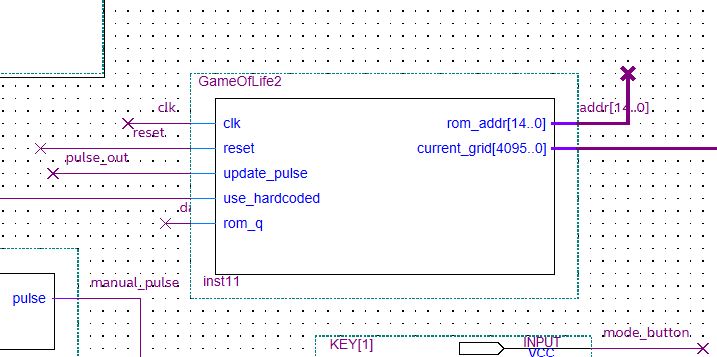
\includegraphics[width=0.90\textwidth]{gameoflife2_intopbdf.png}
		\caption{Diagrama BDF mostrando a instância do módulo \texttt{GameOfLife2}
			no \textit{top-level}, com suas conexões de clock, reset, pulso de
			atualização, ROM e saída da grade.}
		\label{fig:gameoflife_bdf}
	\end{figure}
	
	\subsection{Diagrama BDF do Módulo \texttt{VGA\_SYNC} no \textit{Top-Level}}
	
	A Figura~\ref{fig:vga_sync_bdf} apresenta o diagrama BDF do controlador
	\texttt{VGA\_SYNC} integrado ao \textit{top-level}, mostrando os sinais de
	sincronismo e coordenadas gerados para o restante do sistema.
	
	\begin{figure}[H]
		\centering
		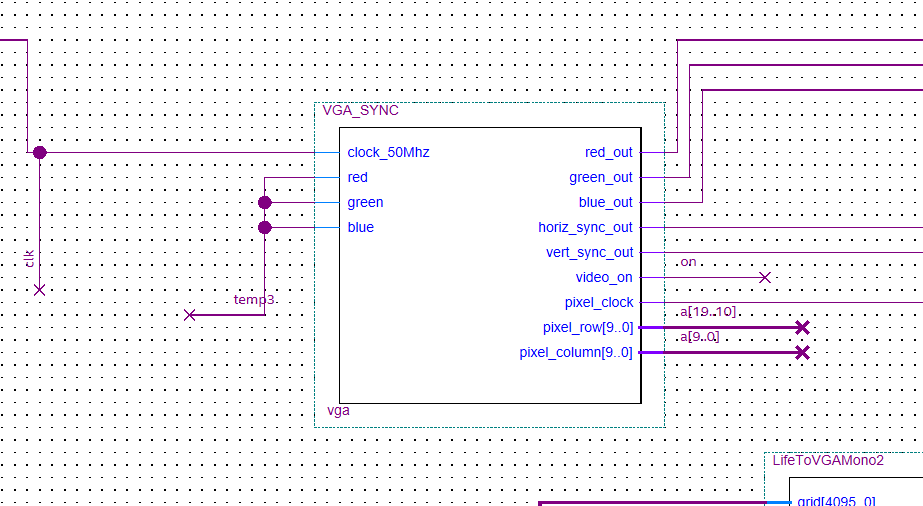
\includegraphics[width=0.90\textwidth]{vga_sync_in_top_bdf.png}
		\caption{Diagrama BDF do controlador \texttt{VGA\_SYNC} no \textit{top-level},
			evidenciando as saídas de sincronismo horizontal e vertical, pixel
			clock, coordenadas de varredura e sinal \texttt{video\_on}.}
		\label{fig:vga_sync_bdf}
	\end{figure}
	
	\subsection{Diagrama BDF da Memória ROM}
	
	A Figura~\ref{fig:rom_bdf} apresenta o diagrama BDF da memória ROM utilizada
	para armazenar o padrão inicial alternativo de 4096 células.
	
	\begin{figure}[H]
		\centering
		
\includegraphics[width=0.70\textwidth]{rom_bdf.png}
		\caption{Diagrama BDF do módulo \texttt{rom} no Quartus Prime, com entrada
			de clock e endereço de 15 bits, e saída de dado de 1 bit por ciclo.}
		\label{fig:rom_bdf}
	\end{figure}
	
	% ============================================================
	%  SEÇÃO 4 — DISCUSSÃO DOS RESULTADOS
	% ============================================================
	\section{Discussão dos Resultados}
	
	\subsection{Comportamento do Canhão de Planadores de Gosper}
	
	Com \texttt{SW[0] = 1} (padrão \textit{hardcoded}), o sistema exibe o Canhão de
	Planadores de Gosper imediatamente após o reset. A Figura~\ref{fig:game_example}
	apresenta o estado do autômato capturado durante a execução na placa DE1, exibido
	no monitor VGA. É possível observar a estrutura central oscilante do canhão e os
	planadores emitidos deslocando-se diagonalmente em direção ao canto inferior
	direito da grade.
	
	\begin{figure}[H]
		\centering
		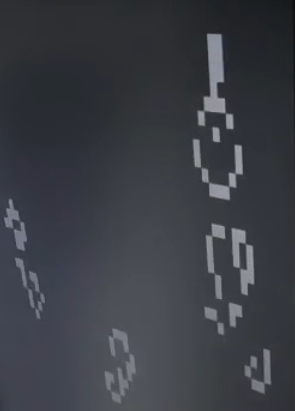
\includegraphics[width=0.75\textwidth]{game_picture_example.png}
		\caption{Estado do Jogo da Vida de Conway exibido no monitor VGA durante
			execução na placa DE1, com o Canhão de Planadores de Gosper como padrão
			\textit{hardcoded} (\texttt{SW[0] = 1}). Células vivas aparecem em branco
			e células mortas em preto.}
		\label{fig:game_example}
	\end{figure}
	
	O comportamento observável no monitor VGA confirma as propriedades teóricas do
	padrão: a estrutura central oscila com período 30 gerações e emite planadores
	que se deslocam diagonalmente em direção ao canto inferior direito da grade.
	Após atingirem a borda fixa, os planadores são absorvidos e desaparecem, sem
	interferir com o canhão central.
	
	O modo manual (\texttt{SW[1] = 1}) permite verificar geração a geração a
	evolução do padrão, confirmando que as regras de transição são aplicadas
	corretamente para todas as células do interior da grade.
	
	\subsection{Paralelismo Massivo e Implicações para Síntese}
	
	A abordagem de atualização paralela da grade completa em um único ciclo de clock
	tem implicações significativas para o processo de síntese. O sintetizador do
	Quartus Prime expande os laços \texttt{for} aninhados em lógica combinacional
	para todas as 3.844 células interiores da grade (62$\times$62), resultando em
	um circuito com:
	
	\begin{itemize}
		\item 3.844 somadores de 8 bits de 1 bit cada (ou equivalentes com 8 portas
		lógicas de adição);
		\item 3.844 comparadores para os valores 2 e 3 do contador de vizinhos;
		\item 3.844 multiplexadores para a função de transição;
		\item 4.096 flip-flops de 1 bit para o registrador \texttt{current\_grid}.
	\end{itemize}
	
	Esta lógica massiva demanda um número elevado de \textit{Logic Elements} (LEs)
	da Cyclone II, possivelmente próximo ou acima da capacidade do EP2C20F484C7
	(18.752 LEs). Em caso de excesso de recursos, o Quartus Prime pode não completar
	a síntese ou pode reduzir a frequência máxima de operação abaixo de 50~MHz.
	Uma solução alternativa, caso os recursos sejam insuficientes, seria adotar
	a abordagem de pipeline seriado com \textit{line buffers}, similar à Prática
	anterior, reduzindo o custo de lógica a expensas de maior complexidade de
	controle.
	
	\subsection{Controle de Velocidade e Interação com o Usuário}
	
	O esquema de controle duplo (automático/manual) mostrou-se funcional e intuitivo.
	No modo automático, a taxa de 10 gerações por segundo é adequada para observar
	a dinâmica global do autômato --- rápida o suficiente para perceber movimento,
	lenta o suficiente para identificar estruturas. O modo manual permite análise
	detalhada de transições específicas, essencial para verificar a correção da
	implementação.
	
	O módulo \texttt{button\_pulse}, ao detectar apenas a borda de descida do botão
	(e não o nível), elimina o problema de múltiplos acionamentos por um único
	pressionamento (\textit{key bounce} em nível), embora o \textit{bounce} em borda
	ainda possa causar múltiplos pulsos em um único pressionamento físico. Para uma
	implementação robusta, seria necessário adicionar um circuito de
	\textit{debouncing} por contador.
	
	\subsection{Mapeamento VGA e Qualidade Visual}
	
	O fator de escala $10 \times 7$ pixels por célula produz células retangulares
	(não quadradas) na tela, o que é uma aproximação aceitável dado que o fator de
	aspecto ($10/7 \approx 1{,}43$) é próximo de 1. Células quadradas exigiria um
	fator de escala de $7 \times 7$ (cobrindo apenas $448 \times 448$ pixels) ou
	$10 \times 10$ (exigindo resolução de $640 \times 640$, maior que o VGA padrão).
	A solução adotada maximiza o uso da tela disponível dentro das restrições do
	padrão VGA 640$\times$480.
	
	\subsection{Demonstração em Vídeo}
	
	O funcionamento completo do sistema --- incluindo a evolução do Canhão de
	Planadores de Gosper em modo automático, o avanço manual geração a geração
	e a exibição em tempo real no monitor VGA --- foi registrado em vídeo e está
	disponível publicamente no YouTube:
	
	\begin{center}
		\url{https://youtu.be/mJRZNuSQj3Y}
	\end{center}
	
	\noindent O vídeo demonstra os diferentes modos de operação selecionáveis pelas
	chaves e botões da placa DE1, evidenciando o comportamento correto do autômato
	celular e o sincronismo entre a lógica de atualização e a saída VGA.
	
	% ============================================================
	%  SEÇÃO 5 — CONCLUSÕES
	% ============================================================
	\section{Conclusões}
	
	Esta prática demonstrou com sucesso a implementação do Jogo da Vida de Conway em
	FPGA, cobrindo desde a modelagem do autômato celular em Verilog até a exibição
	em tempo real no monitor VGA. As principais conclusões são:
	
	\begin{enumerate}
		\item \textbf{Autômatos celulares são naturalmente paralelos em FPGA:} A
		independência entre as atualizações de células distintas na mesma geração
		permite que todo o cálculo da próxima geração seja realizado em lógica
		combinacional paralela, completando uma geração por ciclo de clock. Esta
		é a exploração mais direta possível do paralelismo espacial oferecido pela
		arquitetura reconfigurável do FPGA.
		
		\item \textbf{A separação de clock de atualização e clock de exibição é
			essencial:} A grade evolui a 10~Hz (controlada pelo \texttt{clock\_divider}),
		enquanto o VGA varre a tela a 60~Hz com pixel clock de 25~MHz. O uso de
		registradores síncronos para \texttt{current\_grid} e leitura combinacional
		pelo \texttt{LifeToVGAMono2} garante que qualquer quadro VGA exibe um estado
		consistente da grade, sem artefatos de escrita parcial.
		
		\item \textbf{A interface de usuário com múltiplos modos enriquece a
			observação:} A combinação de reset, seleção de padrão inicial, modo
		automático/manual e avanço por botão transforma o sistema em uma plataforma
		interativa de exploração do autômato, adequada tanto para verificação de
		correção quanto para demonstração didática do comportamento emergente do
		Jogo da Vida.
		
		\item \textbf{O Canhão de Gosper valida a implementação:} A exibição correta
		do canhão de Gosper --- com seu período de 30 gerações e emissão regular de
		planadores --- constitui uma validação funcional robusta da implementação das
		regras de Conway, pois qualquer erro nas regras de transição produziria um
		comportamento visivelmente incorreto deste padrão bem-documentado.
		
		\item \textbf{A abordagem paralela pura tem custo de síntese elevado:} A
		expansão de laços \texttt{for} aninhados para 3.844 células em lógica
		combinacional é a principal limitação de escalabilidade do projeto. Para
		grades maiores (ex.: 128$\times$128 ou 256$\times$256), a abordagem de
		pipeline seriado com \textit{line buffers} --- similar à Prática anterior
		--- seria necessária para manter o projeto dentro dos recursos disponíveis
		na FPGA.
	\end{enumerate}
	
	% ============================================================
	%  SEÇÃO 6 — REFERÊNCIAS BIBLIOGRÁFICAS (ABNT)
	% ============================================================
	\section{Referências Bibliográficas}
	
	\begin{thebibliography}{9}
		
		\bibitem{conway}
		GARDNER, Martin.
		\textbf{Mathematical Games: The fantastic combinations of John Conway's new
			solitaire game ``life''}.
		\textit{Scientific American}, v. 223, n. 4, p. 120--123, out. 1970.
		
		\bibitem{gosper}
		BERLEKAMP, Elwyn R.; CONWAY, John H.; GUY, Richard K.
		\textbf{Winning Ways for Your Mathematical Plays}.
		2. ed. Natick: A K Peters, 2004. v. 4.
		
		\bibitem{lifeWiki}
		LIFEWIKI.
		\textbf{Gosper glider gun}.
		Disponível em: \url{https://conwaylife.com/wiki/Gosper_glider_gun}.
		Acesso em: 25 mai. 2026.
		
		\bibitem{embarcados1}
		EMBARCADOS.
		\textbf{Controlador VGA --- Parte 1}.
		Disponível em: \url{https://embarcados.com.br/controlador-vga-parte-1/}.
		Acesso em: 25 mai. 2026.
		
		\bibitem{embarcados2}
		EMBARCADOS.
		\textbf{Controlador VGA --- Parte 2}.
		Disponível em: \url{https://embarcados.com.br/controlador-vga-parte-2/}.
		Acesso em: 25 mai. 2026.
		
		\bibitem{quartus}
		INTEL CORPORATION.
		\textbf{Quartus Prime Standard Edition Handbook}.
		Disponível em: \url{https://www.intel.com/content/www/us/en/programmable/documentation/}.
		Acesso em: 25 mai. 2026.
		
		\bibitem{roteiro6}
		PEDRINO, Emerson Carlos.
		\textbf{Roteiro da Prática 6: Jogo da Vida em FPGA com Arquitetura Pipeline}.
		São Carlos: UFSCar --- Departamento de Computação, 2026.
		Disponível em: $\langle$\url{https://ava.ufscar.br}$\rangle$. Acesso em: 25 mai. 2026.
		
		\bibitem{patterson}
		PATTERSON, David A.; HENNESSY, John L.
		\textbf{Organização e Projeto de Computadores: a Interface Hardware/Software}.
		5. ed. Rio de Janeiro: Elsevier, 2017.
		
		\bibitem{thomas}
		THOMAS, Donald E.; MOORBY, Philip R.
		\textbf{The Verilog Hardware Description Language}.
		5. ed. New York: Springer, 2002.
		
	\end{thebibliography}
	
	\end{document}